% exchange_scales.tex - standalone build of paper fig:exchange-scales
% (tikzpicture copied verbatim from paper/main.tex lines 858-1056).
% Rebuild with: pdflatex exchange_scales.tex
\documentclass[tikz,border=6pt]{standalone}
\usetikzlibrary{arrows.meta,decorations.pathreplacing}
\begin{document}
	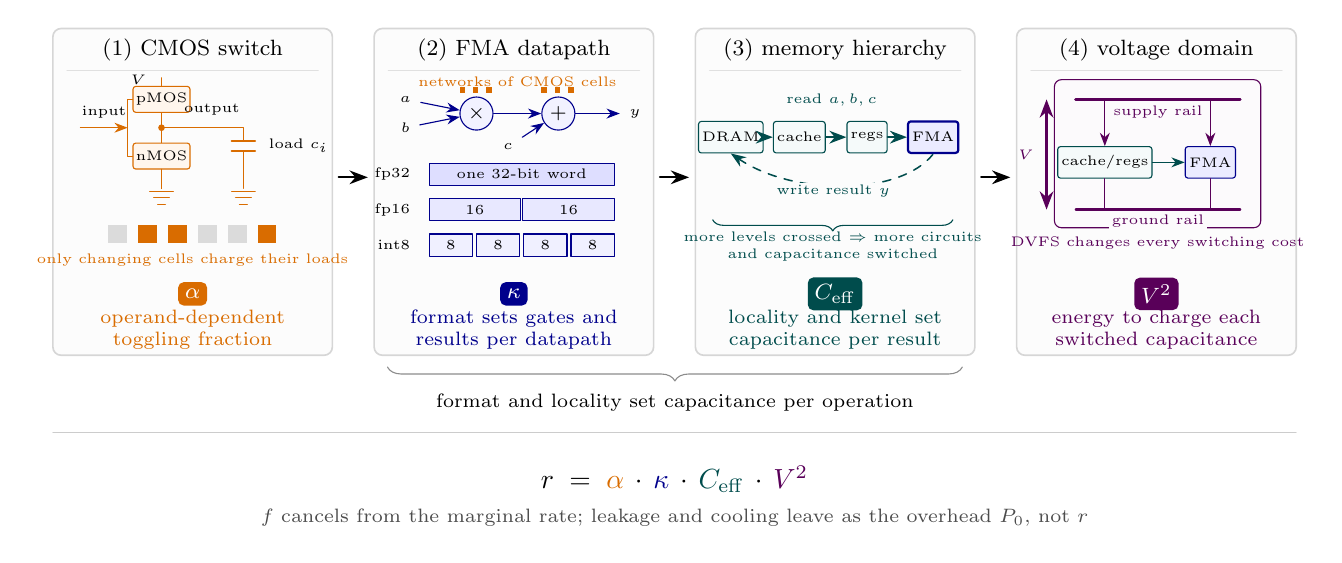
\begin{tikzpicture}[
		>=Stealth, line join=round, line cap=round,
		panel/.style={draw=black!16, fill=black!1, rounded corners=3pt,
			line width=0.6pt},
		badge/.style={rounded corners=2pt, inner sep=2.5pt,
			font=\footnotesize},
		note/.style={font=\scriptsize, align=center},
		title/.style={font=\footnotesize},
		tiny/.style={font=\tiny},
		mos/.style={font=\tiny, draw=orange!85!black, fill=orange!7,
			rounded corners=1pt, minimum width=0.62cm, minimum height=0.33cm,
			inner sep=1pt},
		logic/.style={font=\scriptsize, draw=blue!55!black, fill=blue!5,
			circle, minimum size=0.42cm, inner sep=0pt},
		fma/.style={font=\tiny, draw=blue!55!black, fill=blue!8,
			rounded corners=1pt, minimum height=0.4cm, inner sep=1.5pt},
		mem/.style={font=\tiny, draw=teal!60!black, fill=teal!4,
			rounded corners=1pt, minimum height=0.4cm, inner sep=1.3pt}]

		% Four equal panels form a physical zoom-out: complementary MOSFETs make
		% logic, logic makes a width-selected FMA, the FMA exchanges operands with
		% the memory hierarchy, and one voltage supply energises the whole path.
		% ============ (1) complementary CMOS switching --- alpha ============
		\begin{scope}[shift={(0,0)}]
			\draw[panel] (0,0.1) rectangle (3.55,4.25);
			\node[title] at (1.775,3.98) {(1) CMOS switch};
			\draw[black!12] (0.18,3.72) -- (3.37,3.72);

			% A deliberately simple CMOS inverter: the complementary devices share
			% their input and output, and drive one effective load capacitance.
			\node[mos] (pmos) at (1.38,3.35) {pMOS};
			\node[mos] (nmos) at (1.38,2.63) {nMOS};
			\draw[orange!85!black, line width=0.65pt]
				(1.38,3.62) -- (pmos)
				(pmos) -- (1.38,2.99) -- (nmos) -- (1.38,2.22);
			\node[tiny, black, anchor=east] at (1.31,3.60) {\(V\)};
			\draw[orange!85!black] (1.23,2.18) -- (1.53,2.18)
				(1.28,2.10) -- (1.48,2.10) (1.33,2.02) -- (1.43,2.02);
			\fill[orange!85!black] (1.38,2.99) circle (1.2pt);
			\draw[->, orange!85!black] (0.35,2.99) -- (0.95,2.99)
				node[tiny, black, midway, above] {input};
			\draw[orange!85!black] (0.95,2.99) -- (0.95,3.35) -- (pmos.west)
				(0.95,2.99) -- (0.95,2.63) -- (nmos.west);
			\draw[orange!85!black] (1.38,2.99) -- (2.42,2.99) -- (2.42,2.82);
			\draw[orange!85!black, line width=0.7pt] (2.27,2.82) -- (2.57,2.82);
			\draw[orange!85!black, line width=0.7pt] (2.27,2.69) -- (2.57,2.69);
			\draw[orange!85!black] (2.42,2.69) -- (2.42,2.22);
			\draw[orange!85!black] (2.27,2.18) -- (2.57,2.18)
				(2.32,2.10) -- (2.52,2.10) (2.37,2.02) -- (2.47,2.02);
			\node[tiny, anchor=west] at (2.62,2.76) {load \(c_i\)};
			\node[tiny, anchor=south] at (2.02,3.02) {output};

			% An operand changes only some of the many cells in a datapath.
			\foreach \x/\c in {0.82/gray!28,1.20/orange!85!black,
				1.58/orange!85!black,1.96/gray!28,2.34/gray!28,2.72/orange!85!black}
				\fill[\c] (\x-0.12,1.52) rectangle (\x+0.12,1.76);
			\node[tiny, text=orange!85!black] at (1.775,1.31)
				{only changing cells charge their loads};
			\node[badge, fill=orange!85!black, text=white] at (1.775,0.88)
				{\(\alpha\)};
			\node[note, text=orange!85!black] at (1.775,0.43)
				{operand-dependent\\toggling fraction};
		\end{scope}

		\draw[->, thick] (3.63,2.36) -- (4.00,2.36);

		% ============ (2) bit-width-selected FMA --- kappa ============
		\begin{scope}[shift={(4.08,0)}]
			\draw[panel] (0,0.1) rectangle (3.55,4.25);
			\node[title] at (1.775,3.98) {(2) FMA datapath};
			\draw[black!12] (0.18,3.72) -- (3.37,3.72);

			% CMOS logic implements a multiplier followed by an accumulator.
			\node[tiny] (ain) at (0.40,3.35) {\(a\)};
			\node[tiny] (bin) at (0.40,2.99) {\(b\)};
			\node[logic] (mul) at (1.30,3.17) {\(\times\)};
			\node[logic] (add) at (2.34,3.17) {\(+\)};
			\node[tiny] (cin) at (1.70,2.75) {\(c\)};
			\draw[->, blue!55!black] (ain) -- (mul);
			\draw[->, blue!55!black] (bin) -- (mul);
			\draw[->, blue!55!black] (mul) -- (add);
			\draw[->, blue!55!black] (cin) -- (add);
			\draw[->, blue!55!black] (add) -- (3.12,3.17)
				node[tiny, black, right] {\(y\)};
			\foreach \x in {1.12,1.29,1.46,2.16,2.33,2.50}
				\fill[orange!85!black]
					(\x-0.035,3.435) rectangle (\x+0.035,3.505);
			\node[tiny, text=orange!85!black] at (1.82,3.58) {networks of CMOS cells};

			% A fixed-width fabric can hold one wide word or several narrow words.
			% The partitions make the numeric encoding and packing explicit.
			\node[tiny, anchor=east] at (0.58,2.40) {fp32};
			\draw[blue!55!black, fill=blue!13] (0.70,2.26) rectangle (3.05,2.54);
			\node[tiny] at (1.875,2.40) {one 32-bit word};
			\node[tiny, anchor=east] at (0.58,1.95) {fp16};
			\foreach \x in {0.70,1.89}
				\draw[blue!55!black, fill=blue!9] (\x,1.81) rectangle (\x+1.16,2.09);
			\node[tiny] at (1.28,1.95) {16};
			\node[tiny] at (2.47,1.95) {16};
			\node[tiny, anchor=east] at (0.58,1.50) {int8};
			\foreach \x in {0.70,1.30,1.90,2.50}
				\draw[blue!55!black, fill=blue!6] (\x,1.36) rectangle (\x+0.55,1.64);
			\foreach \x in {0.975,1.575,2.175,2.775}
				\node[tiny] at (\x,1.50) {8};
			\node[badge, fill=blue!55!black, text=white] at (1.775,0.88)
				{\(\kappa\)};
			\node[note, text=blue!55!black] at (1.775,0.43)
				{format sets gates and\\results per datapath};
		\end{scope}

		\draw[->, thick] (7.71,2.36) -- (8.08,2.36);

		% ============ (3) memory hierarchy and operand path --- C_eff ============
		\begin{scope}[shift={(8.16,0)}]
			\draw[panel] (0,0.1) rectangle (3.55,4.25);
			\node[title] at (1.775,3.98) {(3) memory hierarchy};
			\draw[black!12] (0.18,3.72) -- (3.37,3.72);
			\node[mem, minimum width=0.55cm] (dram) at (0.45,2.87) {DRAM};
			\node[mem, minimum width=0.58cm] (cache) at (1.32,2.87) {cache};
			\node[mem, minimum width=0.48cm] (reg) at (2.18,2.87) {regs};
			\node[fma, minimum width=0.52cm, line width=0.8pt]
				(memfma) at (3.02,2.87) {FMA};
			% A value can enter at any level, but must reach the register/FMA end.
			% Equal line widths avoid implying that remote physical wires are thicker;
			% the chain length instead shows how many hierarchy stages are activated.
			\draw[->, teal!60!black, line width=0.7pt] (dram) -- (cache);
			\draw[->, teal!60!black, line width=0.7pt] (cache) -- (reg);
			\draw[->, teal!60!black, line width=0.7pt] (reg) -- (memfma);
			\node[tiny, text=teal!60!black] at (1.73,3.34)
				{read \(a,b,c\)};
			\draw[<-, teal!60!black, dashed, line width=0.55pt]
				(dram.south) .. controls (1.25,2.12) and (2.60,2.12) .. (memfma.south);
			\node[tiny, text=teal!60!black, fill=black!1, inner sep=1pt]
				at (1.75,2.18) {write result \(y\)};
			\draw[decorate, decoration={brace, amplitude=4pt, mirror}, teal!60!black]
				(0.22,1.82) -- (3.27,1.82);
			\node[tiny, text=teal!60!black, align=center] at (1.745,1.48)
				{more levels crossed \(\Rightarrow\) more circuits\\and capacitance switched};
			\node[badge, fill=teal!60!black, text=white] at (1.775,0.88)
				{\(C_{\mathrm{eff}}\)};
			\node[note, text=teal!60!black] at (1.775,0.43)
				{locality and kernel set\\capacitance per result};
		\end{scope}

		\draw[->, thick] (11.79,2.36) -- (12.16,2.36);

		% ============ (4) one supply across that same path --- V^2 ============
		\begin{scope}[shift={(12.24,0)}]
			\draw[panel] (0,0.1) rectangle (3.55,4.25);
			\node[title] at (1.775,3.98) {(4) voltage domain};
			\draw[black!12] (0.18,3.72) -- (3.37,3.72);
			% The repeated memory--FMA motif makes this panel a containing scale of
			% panel (3), rather than a visually unrelated die cartoon.
			\draw[violet!70!black, fill=violet!2, rounded corners=2.5pt]
				(0.48,1.72) rectangle (3.10,3.60);
			\draw[violet!70!black, line width=1.05pt] (0.75,3.35) -- (2.84,3.35);
			\node[tiny, text=violet!70!black, fill=violet!2, inner sep=1pt,
				anchor=north] at (1.795,3.31) {supply rail};
			\draw[violet!70!black, line width=0.8pt] (0.75,1.95) -- (2.84,1.95);
			\node[tiny, text=violet!70!black, fill=violet!2, inner sep=1pt,
				anchor=north] at (1.795,1.92) {ground rail};
			\node[mem] (diemem) at (1.12,2.55) {cache/regs};
			\node[fma] (diefma) at (2.46,2.55) {FMA};
			\draw[->, teal!60!black] (diemem) -- (diefma);
			\draw[->, violet!70!black] (1.12,3.35) -- (diemem);
			\draw[->, violet!70!black] (2.46,3.35) -- (diefma);
			\draw[violet!70!black] (diemem.south) -- (1.12,1.95);
			\draw[violet!70!black] (diefma.south) -- (2.46,1.95);
			\draw[<->, violet!70!black, line width=0.8pt]
				(0.38,1.95) -- (0.38,3.35);
			\node[tiny, text=violet!70!black, anchor=east] at (0.34,2.65)
				{\(V\)};
			\node[tiny, text=violet!70!black] at (1.79,1.52)
				{DVFS changes every switching cost};
			\node[badge, fill=violet!70!black, text=white] at (1.775,0.88)
				{\(V^2\)};
			\node[note, text=violet!70!black] at (1.775,0.43)
				{energy to charge each\\switched capacitance};
		\end{scope}

		% The structural factors together set capacitance per operation.
		\draw[decorate, decoration={brace, amplitude=5pt, mirror}, black!45]
			(4.25,-0.05) -- (11.55,-0.05);
		\node[font=\scriptsize] at (7.90,-0.50)
			{format and locality set capacitance per operation};

		% ============ assembled equation ============
		\draw[black!20] (0,-0.88) -- (15.79,-0.88);
		\node[font=\normalsize] at (7.895,-1.47)
			{\(r \;=\;
			{\color{orange!85!black}\alpha}\,\cdot\,
			{\color{blue!55!black}\kappa}\,\cdot\,
			{\color{teal!60!black}C_{\mathrm{eff}}}\,\cdot\,
			{\color{violet!70!black}V^2}\)};
		\node[font=\scriptsize, text=gray!60!black] at (7.895,-1.96)
			{\(f\) cancels from the marginal rate; leakage and cooling leave as
			the overhead \(P_0\), not \(r\)};

	\end{tikzpicture}%
\end{document}
